\documentclass{article}
\usepackage{amsfonts}
\usepackage{graphicx}
\usepackage[margin=1in]{geometry}
\usepackage{bm}
\usepackage{amsmath}
\usepackage{authblk}
\usepackage{caption}
\usepackage{float}
\renewcommand{\familydefault}{\sfdefault}

\title{Taxonomic Enrichment Analysis with Isometric Log-Ratios}
\author[1,2]{Quang P. Nguyen}
\author[1,2]{Anne G. Hoen}
\author[1]{H. Robert Frost}
\affil[1]{Department of Biomedical Data Science, Geisel School of Medicine at Dartmouth College, Hanover, NH 03755, USA}
\affil[2]{Department of Epidemiology, Geisel School of Medicine at Dartmouth College, Hanover, NH 03755, USA}
\date{}                     %% if you don't need date to appear
\setcounter{Maxaffil}{0}
\renewcommand\Affilfont{\itshape\small}

\begin{document}
\maketitle
\captionsetup[figure]{labelfont={bf},name={Figure},labelsep=period, margin=2cm}

\begin{abstract}
    \noindent High-dimensionality is a challenging problem in analyzing microbiome relative abundance data. Studies commonly alleviate this problem by aggregating variables into sets, most commonly higher order taxonomic classifications. However, such approaches are often naive and does not consider the hypothesis aggregation problem when testing for significance at multiple taxonomic levels. Here we introduced a novel competitive taxonomic enrichment method based on the isometric log-ratio transformation (cILR) for single samples. We demonstrated that our method controls type I error and power for hypothesis testing at the single sample level, as well as providing more robust results than other single sample enrichment methods for differential abundance and prediction tasks.   
\end{abstract}

\section*{Background}
\section*{Methods}
\section*{Results}
In this section we present the performance of our proposed method for three applicable microbiome analysis tasks: sample level enrichment testing, differential abundance testing, and prediction. We obtained these results from both parametric simulations and examples from real data.  
\subsection*{Enrichment testing at the sample level}
There are various settings where researchers want to test for enrichment of certain groups of microbes in an experiment. 
\subsubsection*{Type I error control and power}
We benchmarked type I error on real stool microbiome data from HMP for both 16S and WGS type data. 16S data was taken from the package \emph{HMP16SData} snapshot 2020-10-02. 

\begin{figure}[H]
    \centering
    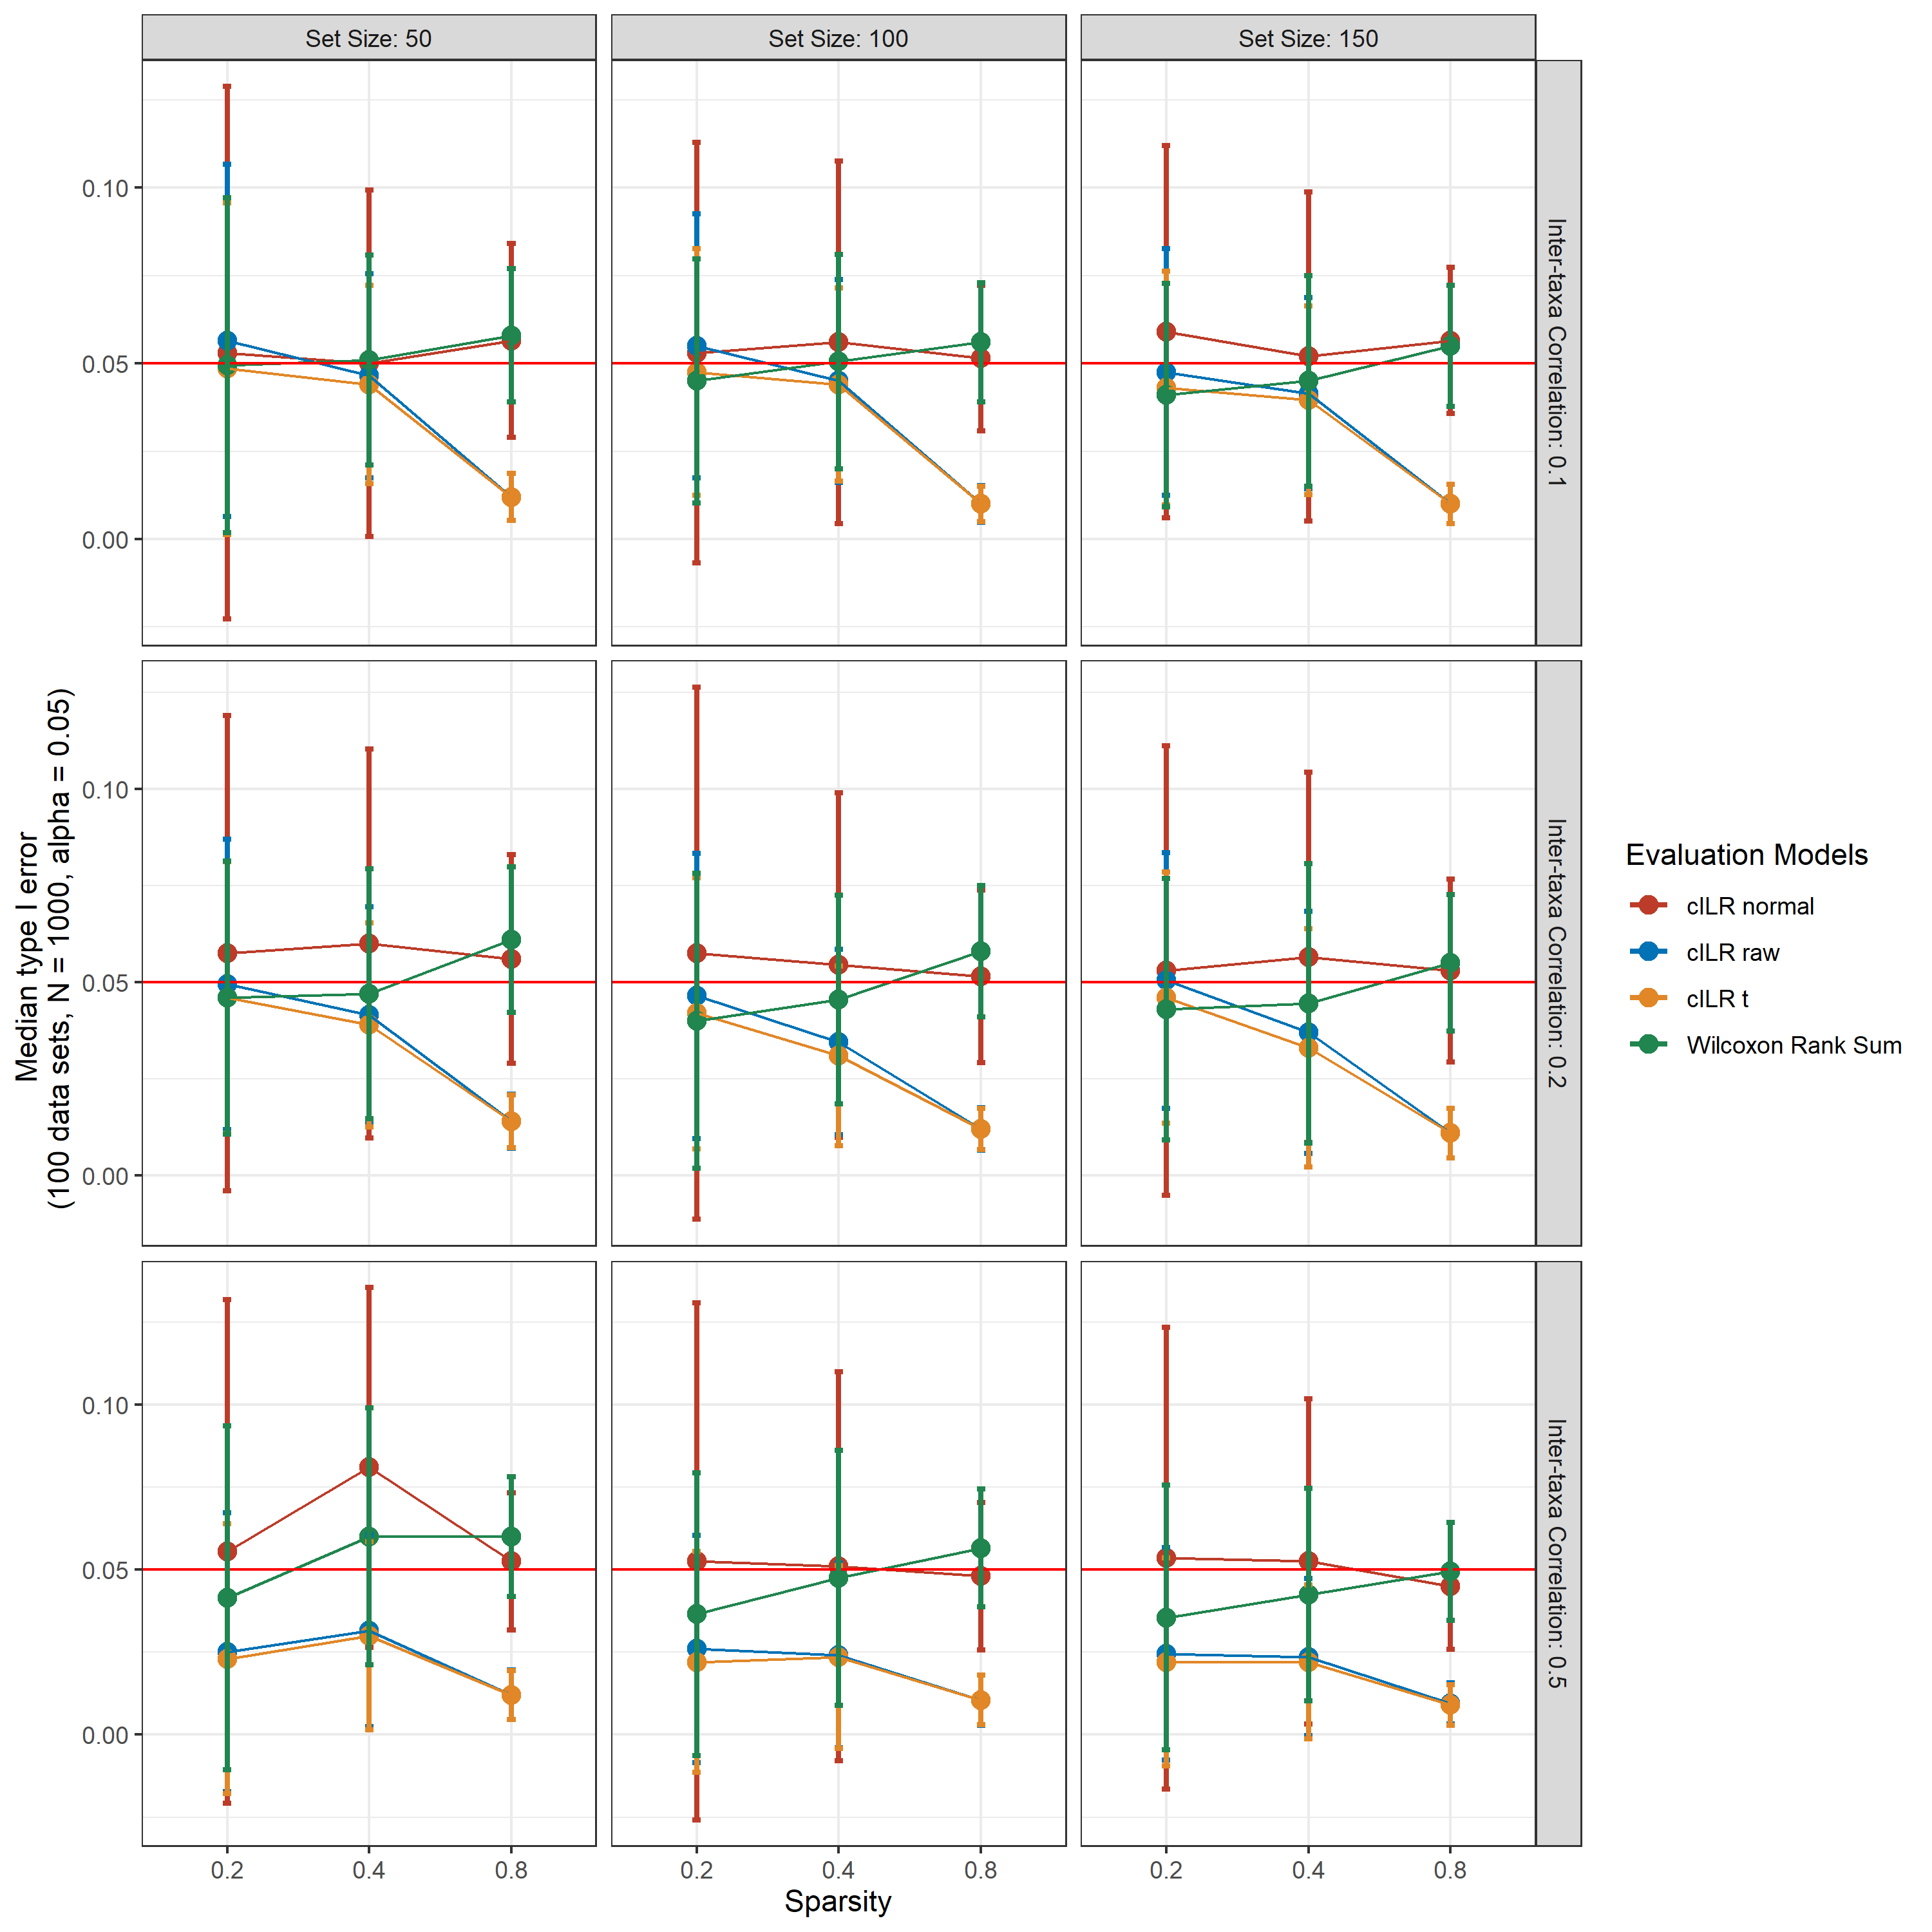
\includegraphics[scale = 0.5]{figures/fdr_single_sample.png}
    \caption{Median type I error rate as a function of data sparsity benchmarked on simulated null microbiome data as enumerated in SI methods. Enrichment of a specified set was tested at the sample level using cILR and the Wilcoxon rank sum test at $\alpha$ of 0.05. Each panel represents different in set size (horizontal) and inter-taxa correlation (vertical)}
\end{figure}

\begin{figure}[H]
    \centering
    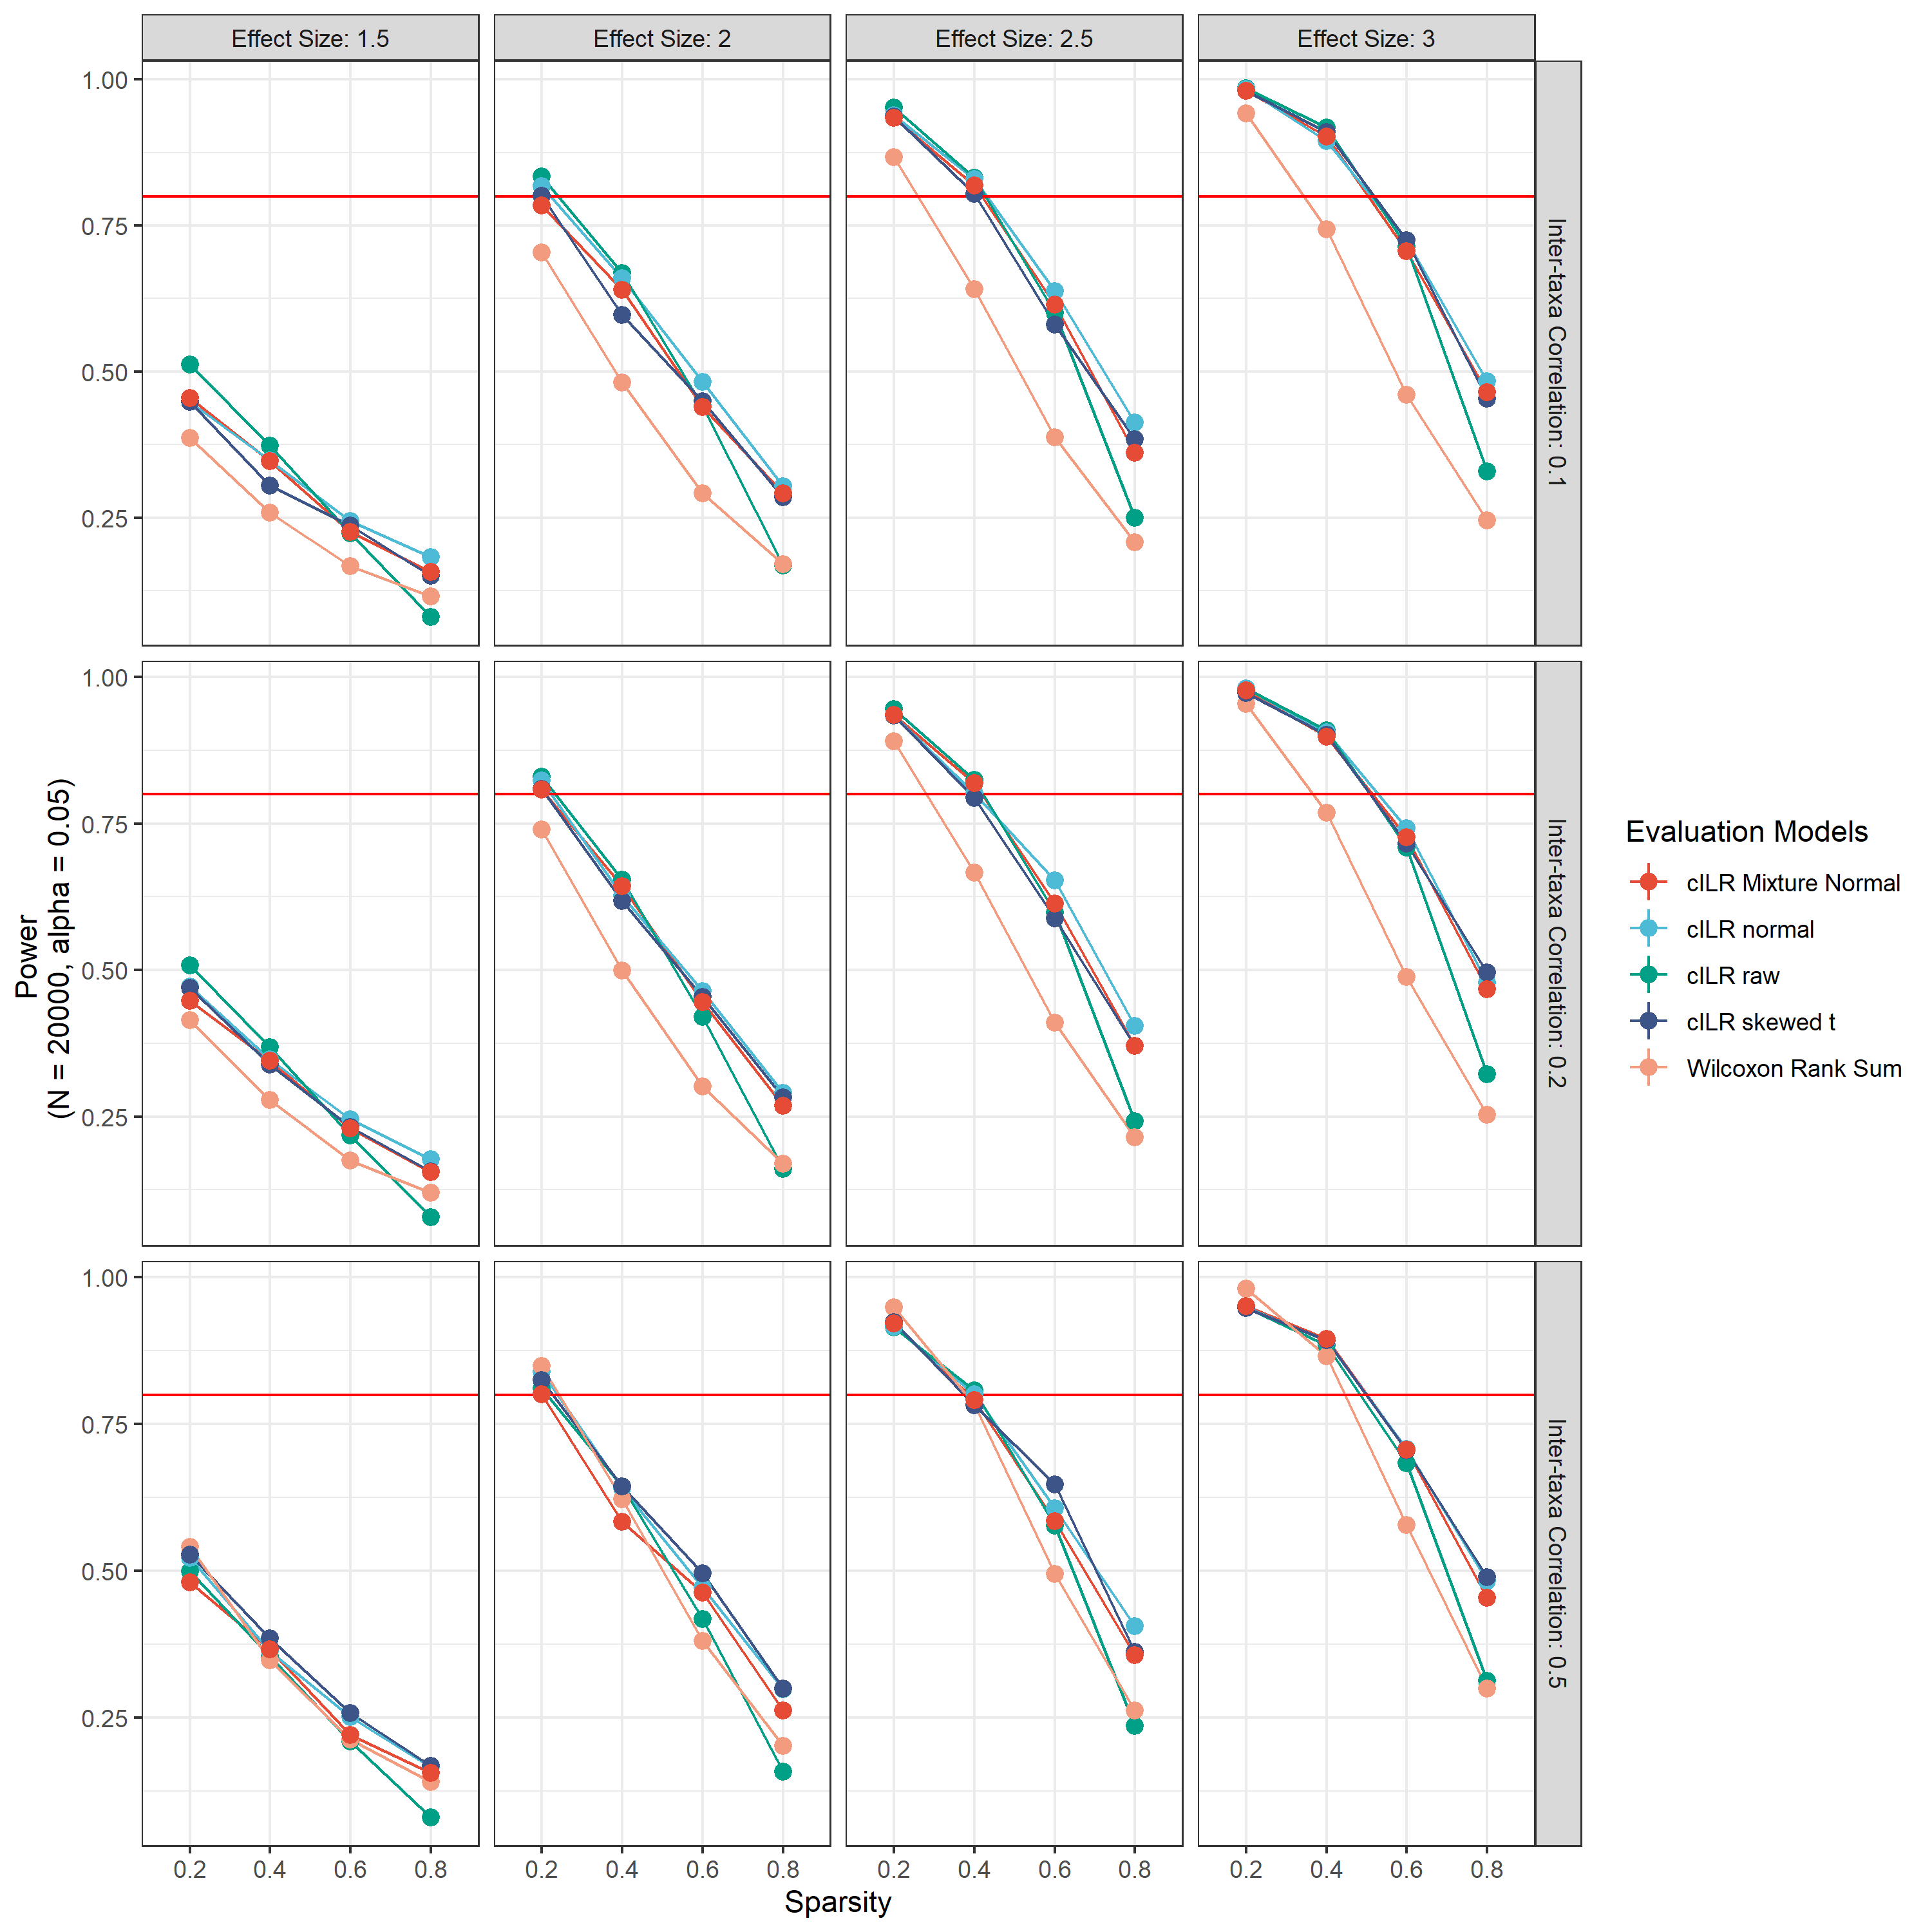
\includegraphics[scale=0.5]{figures/pwr_single_sample.png}
    \caption{Median power as a function of data sparsity benchmarked on simulated microbiome data as enumerated in SI Methods. Enrichment of a specified set was tested at the sample level using cILR and the Wilcoxon rank sum test at $\alpha$ of 0.05. Each panel represents different effect sizes (horizontal) and inter-taxa correlation (vertical).}
\end{figure}

\subsection*{Differential abundance analysis} 
\subsubsection*{Type I error control}
We benchmarked type I error rate of the cILR approach in differential abundance analysis tasks on both real data and numerical experiments. For real data, we utilized 16S rRNA and WGS stool sequencing data from the Human Microbiome project obtained from the packages \emph{HMP16SData} (ver. 1.9.3) and \emph{curatedMetagenomicData} in R. We randomly assigned samples from each data set into two arbitrary groups and evaluated the type I error rate. This procedure was repeated 1000 times. Figure 3 demonstrated these results.\\
We observed 
\begin{figure}[H]
    \centering
    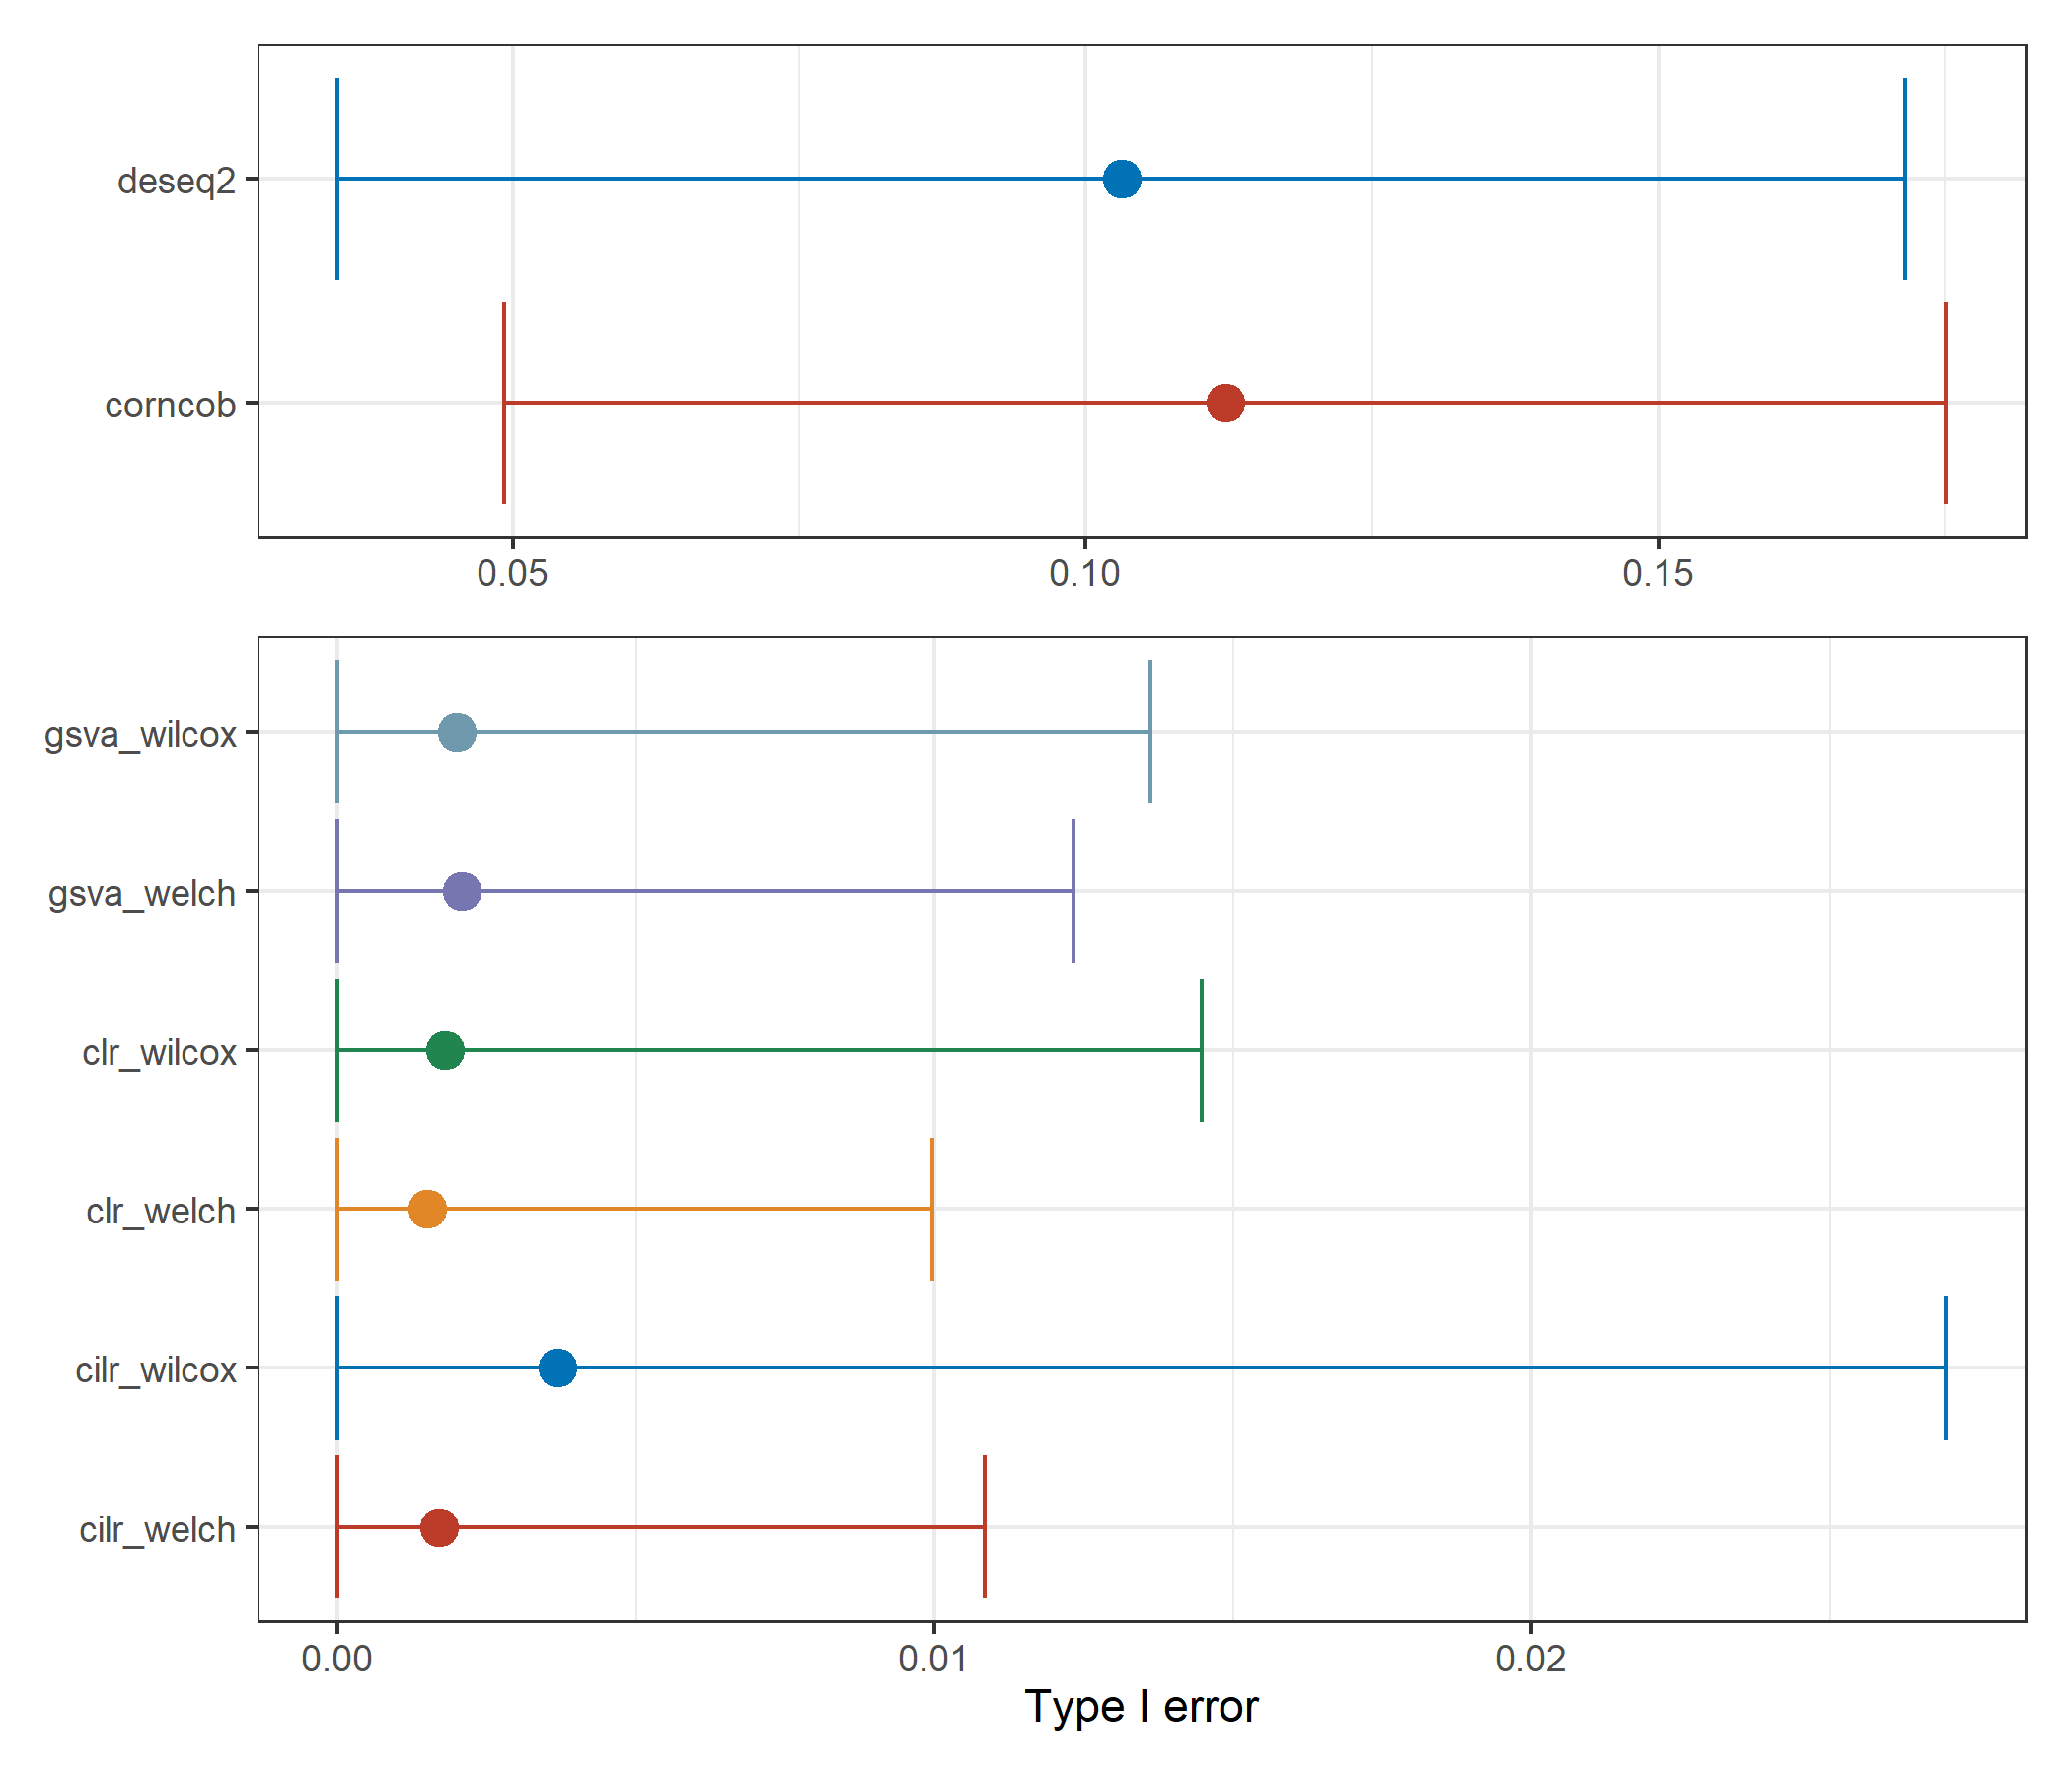
\includegraphics[scale=0.5]{figures/null_16s_da.png}
    \caption{Type I error evaluated on 16S rRNA and WGS stool samples obtained from HMP. Enrichment of genus level taxa sets was tested across different methods where significance was determined at FDR cutoff of 0.05.}
\end{figure}

\newpage
\bibliography{tax_agg}{}
\bibliographystyle{plain}
\end{document}
\end{document}